\documentclass[twocolumn,prb,showpacs,10pt,superscriptaddress]{revtex4-1}
%\documentclass[twocolumn,prb,showpacs,10pt]{article}
\usepackage{textcomp}
\usepackage{amsmath}
\usepackage{amssymb}
\usepackage{subfig}
\def\bra#1{\mathinner{\langle{#1}|}}
\def\ket#1{\mathinner{|{#1}\rangle}}
\def\braket#1{\mathinner{\langle{#1}\rangle}}
\usepackage{color}
\usepackage{multirow}
\usepackage{float} %\floatstyle{boxed} \restylefloat{figure}
\bibliographystyle{apsrev}
\usepackage{fontenc}
\usepackage{graphicx}
\usepackage{graphics}
\usepackage[dvips]{hyperref}
\usepackage[justification=centering]{caption}
%\usepackage[utf8]{inputenc}
%\usepackage{authblk}
\usepackage{lipsum}

\makeatletter
\newcommand{\RNum}[1]{\uppercase\expandafter{\romannumeral #1\relax}}
%\newcommand{\Rmnum}[1]{\expandafter\@slowromancap\romannumeral #1@}
\newcommand*{\rom}[1]{\expandafter\@slowromancap\romannumeral #1@}\newcommand{\rmnum}[1]{\romannumeral #1}
\newcommand{\Rmnum}[1]{\expandafter\@slowromancap\romannumeral #1@}
%\newcommand{\rmnum}[1]{\romannumeral #1}
%\newcommand{\Rmnum}[1]{\expandafter\@slowromancap\romannumeral #1@}

\begin{document}

\title{Electron transport study in coherent tunneling through cyclic Ru/Os(PPh$_{2}$)$_{8}$(C$_{2}$H$_{4}$)$_{4}$ bis(pyridylacetylide) complexes}
\author{Xin Zhao}
\affiliation{Institute for Theoretical Physics, TU Wien - Vienna University of Technology, Wiedner Hauptstrasse 8-10, A-1040 Vienna, Austria}
\author{Robert Stadler}
\email[Email:]{robert.stadler@tuwien.ac.at}
\affiliation{Institute for Theoretical Physics, TU Wien - Vienna University of Technology, Wiedner Hauptstrasse 8-10, A-1040 Vienna, Austria}

\date{\today}

\begin{abstract}

In our theoretical study where we combine an nonequilibrium Green's function (NEGF) approach with density functional theory (DFT) we investigate branched compounds containing Ru or Os metal complexes in two branches, which due to their identical or different metal centers are designed to allow for local charging induced or in-built asymmetry. 
In these compounds the metal atoms are connected to pyridyl anchor groups via acetylenic spacer groups and benzene rings in a meta-connection where we also compare our results with those obtained for the respective single branch molecules. 
We find there is no destructive quantum interference (DQI) feature in the transmission function within the interesting region (near by the Fermi level) for the investigated molecules, neither in their neutral states, nor in their charged states. 
Based on our knowledge for previously studied molecules containing ferroecene moieties we map the structural characteristics of the range of molecules onto a simplified tight-binding model, we identify the main differences between the longer cyclic molecules and the previously investigated ferrocene compounds in order to clarify the structural sources for DQI. 
We also find that local charging on one of the branches only changes the conductance slightly (by about one order of magnitude) which we explain in terms of the spatial distributions of the relevant molecular orbitals for the branched compounds.
\end{abstract}

\maketitle
\subsection{Introduction}

Under the restrictions of low bias current flowing through small molecules absorbed to metal electrodes in ultrahigh vacuum at very low temperature, the field of
single-molecular electronics ~\cite{ratner,loertscher} has become accessible for an nonequilibrium Green's function (NEGF) approach combined with density functional theory (DFT), which allows for an atomic interpretation of experimental results in a mechanical break-junction (MCBJ) or scanning tunneling microscope (STM) setup ~\cite{Thygesen 2005, C. Joachim 1995, M. A. Reed 1997,J. Reichert 2002, R. H. M. Smit 2002}. 
Destructive quantum interference (DQI) effects ~\cite{mayor,lambert1} allow for the design of logical gates ~\cite{graphical1} and memory cells ~\cite{memory} in single molecule electronics as well as the implementation of thermoelectric devices ~\cite{fano,lambert2}, since DQI is supposed to significantly reduce the conductance in conjugated $\pi$ systems where this feature is observable at room temperature ~\cite{molen}.

Experimentally, the design and synthesis of branched compounds containing ferrocene moieties in each branch has been proposed ~\cite{tim} for the purpose of creating single molecule junctions, where the combination of quantum interference effects with redox gating for coherent electron tunneling as well as the electrostatic correlation between spatially distinct redox centers for electron hopping ~\cite{Georg 2015} can be explored. Theoretically a detailed analysis of branched compounds containing ferrocene centers has been published in our previous work ~\cite{Xin2017}. In order to confirm the generality of this analysis we apply the same models and methods to cyclic Ru/Os(PPh$_{2}$)$_{8}$(C$_{2}$H$_{4}$)$_{4}$ bis(pyridylacetylide) molecules, where we use the notation of Ru/Os, Os/Os, Ru/Ru for the complexes containing symmetrical and asymmetrical branches. There are experimental and theoretical studies ~\cite{Georg 2015, Schwarz 2015} about coherent tunneling and electron hopping for Ru redox-active single-molecule junctions. Ref. ~\cite{Georg 2015} is focus on the comparison between coherent tunneling and hopping mechanisms in dependence of junction length for ruthenium bis(pyridylacetylide) complexes, and the work in ~\cite{Schwarz 2015} investigated the influence by the charge and spin states of redox-active metal centers on charge transport through single molecules in the transport pathway.
\begin{figure}
\begin{center}
\includegraphics[width=0.5\linewidth,angle=0]{bis-pyridylacetylide-complex.jpg}
\caption{\small Chemical structure for cyclic Ru$_{2}$(PPh$_{2}$)$_{8}$(C$_{2}$H$_{4}$)$_{4}$ bis(pyridylacetylide) complex .
  \label{Fig.chemicalstru}} 
\end{center}
\end{figure}
The simple but effective model we used for the work on branched ferrocene compounds is a combined atomic orbital (AO) fragment orbital (FO) tight-binding (TB) model where we keep only the $p_{\pi}$ AO for each atom in both anchoring groups and one relevant bridge FO. For the molecule in Ref. ~\cite{Xin2017} we found that the through-space coupling between the two anchor groups is the decisive parameter causing DQI effects in the interesting region, i.e. in the gap between the highest occupied molecular orbital (HOMO) and the lowest unoccupied molecular orbital (LUMO) and as close as possible to the Fermi level E${_{F}}$.
In Fig. ~\ref{Fig.chemicalstru} we show a type of molecule where one can create in-built asymmetry and by exchanging one of the redox centers Ru by Os. Due to the longer conjugated groups organic fragments are 
more decoupled from the pyridyl anchors than for the ferrocene compounds we studied in ~\cite{Xin2017}. In this article, we want to address two issues: i) How do the models we used for the branched ferrocene molecules in Ref.~\cite{Xin2017} interpret coherent electron transport for this new type of molecules? ii) Will the decreased through-space couplings due to the longer molecular length have an impact on the occurrence of DQI? 
The paper is organized as follows: In section ~\ref{sec:results} we present transmission functions from NEGF-DFT calculations for all junction geometries and discuss their characteristics features, where comparisons of single and double branched molecules are presented. In section ~\ref{sec:sources} we derive topological tight-binding models from the DFT calculations based on the scheme in our previous study and identify the vanishing through-space coupling between the anchor groups as the decisive parameter for the absence of DQI in all systems investigated in this article. In section ~\ref{Effect of charging} we compare the conductance from NEGF-DFT calculations for the charged systems with the corresponding neutral ones for assessing the usefulness of these double-branched systems as molecular switches. We make a summary and outlook based on our results in section ~\ref{sec:summary}

\section{Computational details for the NEGF-DFT calculations}\label{computationaldetails}

We performed density functional theory (DFT) calculations with a PBE XC-functional within a non equilibrium Green's function (NEGF)-DFT framework ~\cite{M.Brandbyge 2002, Y.Xue 2002, A.R.Rocha 2005, kristian} using a linear combination of atomic orbitals (LCAO) ~\cite{lcao} as basis set on a double zeta level with polarization functions (DZP) in the GPAW code ~\cite{J.Mortensen 2005, J.Enkovaara 2010} for the computation of transmission probabilities, $\mathcal{T}(E)$, grid spacing of 0.2 \AA{} for the sampling of the potential in the Hamiltonian on a real space grid is used.
In our transport calculations, the scattering region is formed by the respective metal organic compounds and three and four layers for the upper and lower fcc gold electrodes, respectively, in a (111) orientation and with a 6 $\times$ 10 gold surface defining the periodically repeated unit cell in the $xy$ plane (transverse directions). The distance between the Au ad-atom attached to the electrodes surface and the N atom of the pyridyl anchor groups is 2.12 \AA{} ~\cite{pyridil1} and a $k$ points sampling corresponding to a 1$\times$2$\times$1 Monkhorst Pack grid is used in scattering region for evaluating $\mathcal{T}(E)$, where the $z$-coordinate is the direction of electron transport through the junction. 

\section{Results and discussion}\label{sec:results}

In Fig. ~\ref{Fig.neutral_big_cyclicmol_junctions} we illustrate the molecular junctions derived from the compound in Fig. ~\ref{Fig.chemicalstru}, 
where the two redox-center are Ru/Os, Os/Os and Ru/Ru, respectively.
The transmission functions $\mathcal{T}(E)$ for these junctions are shown in ~\ref{Fig.big_cyclicmol_tf}. 
In the resulting transmission functions in Fig.~\ref{Fig.big_cyclicmol_tf} the HOMO peaks are close to the Fermi level for all investigated systems, hence we expect the conductance to be dominated by the MOs below $E_{F}$. 
Our definition of DQI is that the transmission through a system with more than one MO around E$_F$ is lower than the sum of the individual contributions of these MOs to $\mathcal{T}(E)$ ~\cite{pyridil3}. 
The exact energetic position of the Fermi energy within the HOMO-LUMO gap, which is also affected by the underestimation of this gap in our calculations due to the PBE parametrization of the XC functional, will have a crucial impact on the quantitative conductance but qualitatively DQI will always result in a significant conductance lowering for the structures where it occurs regardless of the details of the Fermi level alignment ~\cite{victor}.
\begin{figure}[h]
\begin{center}
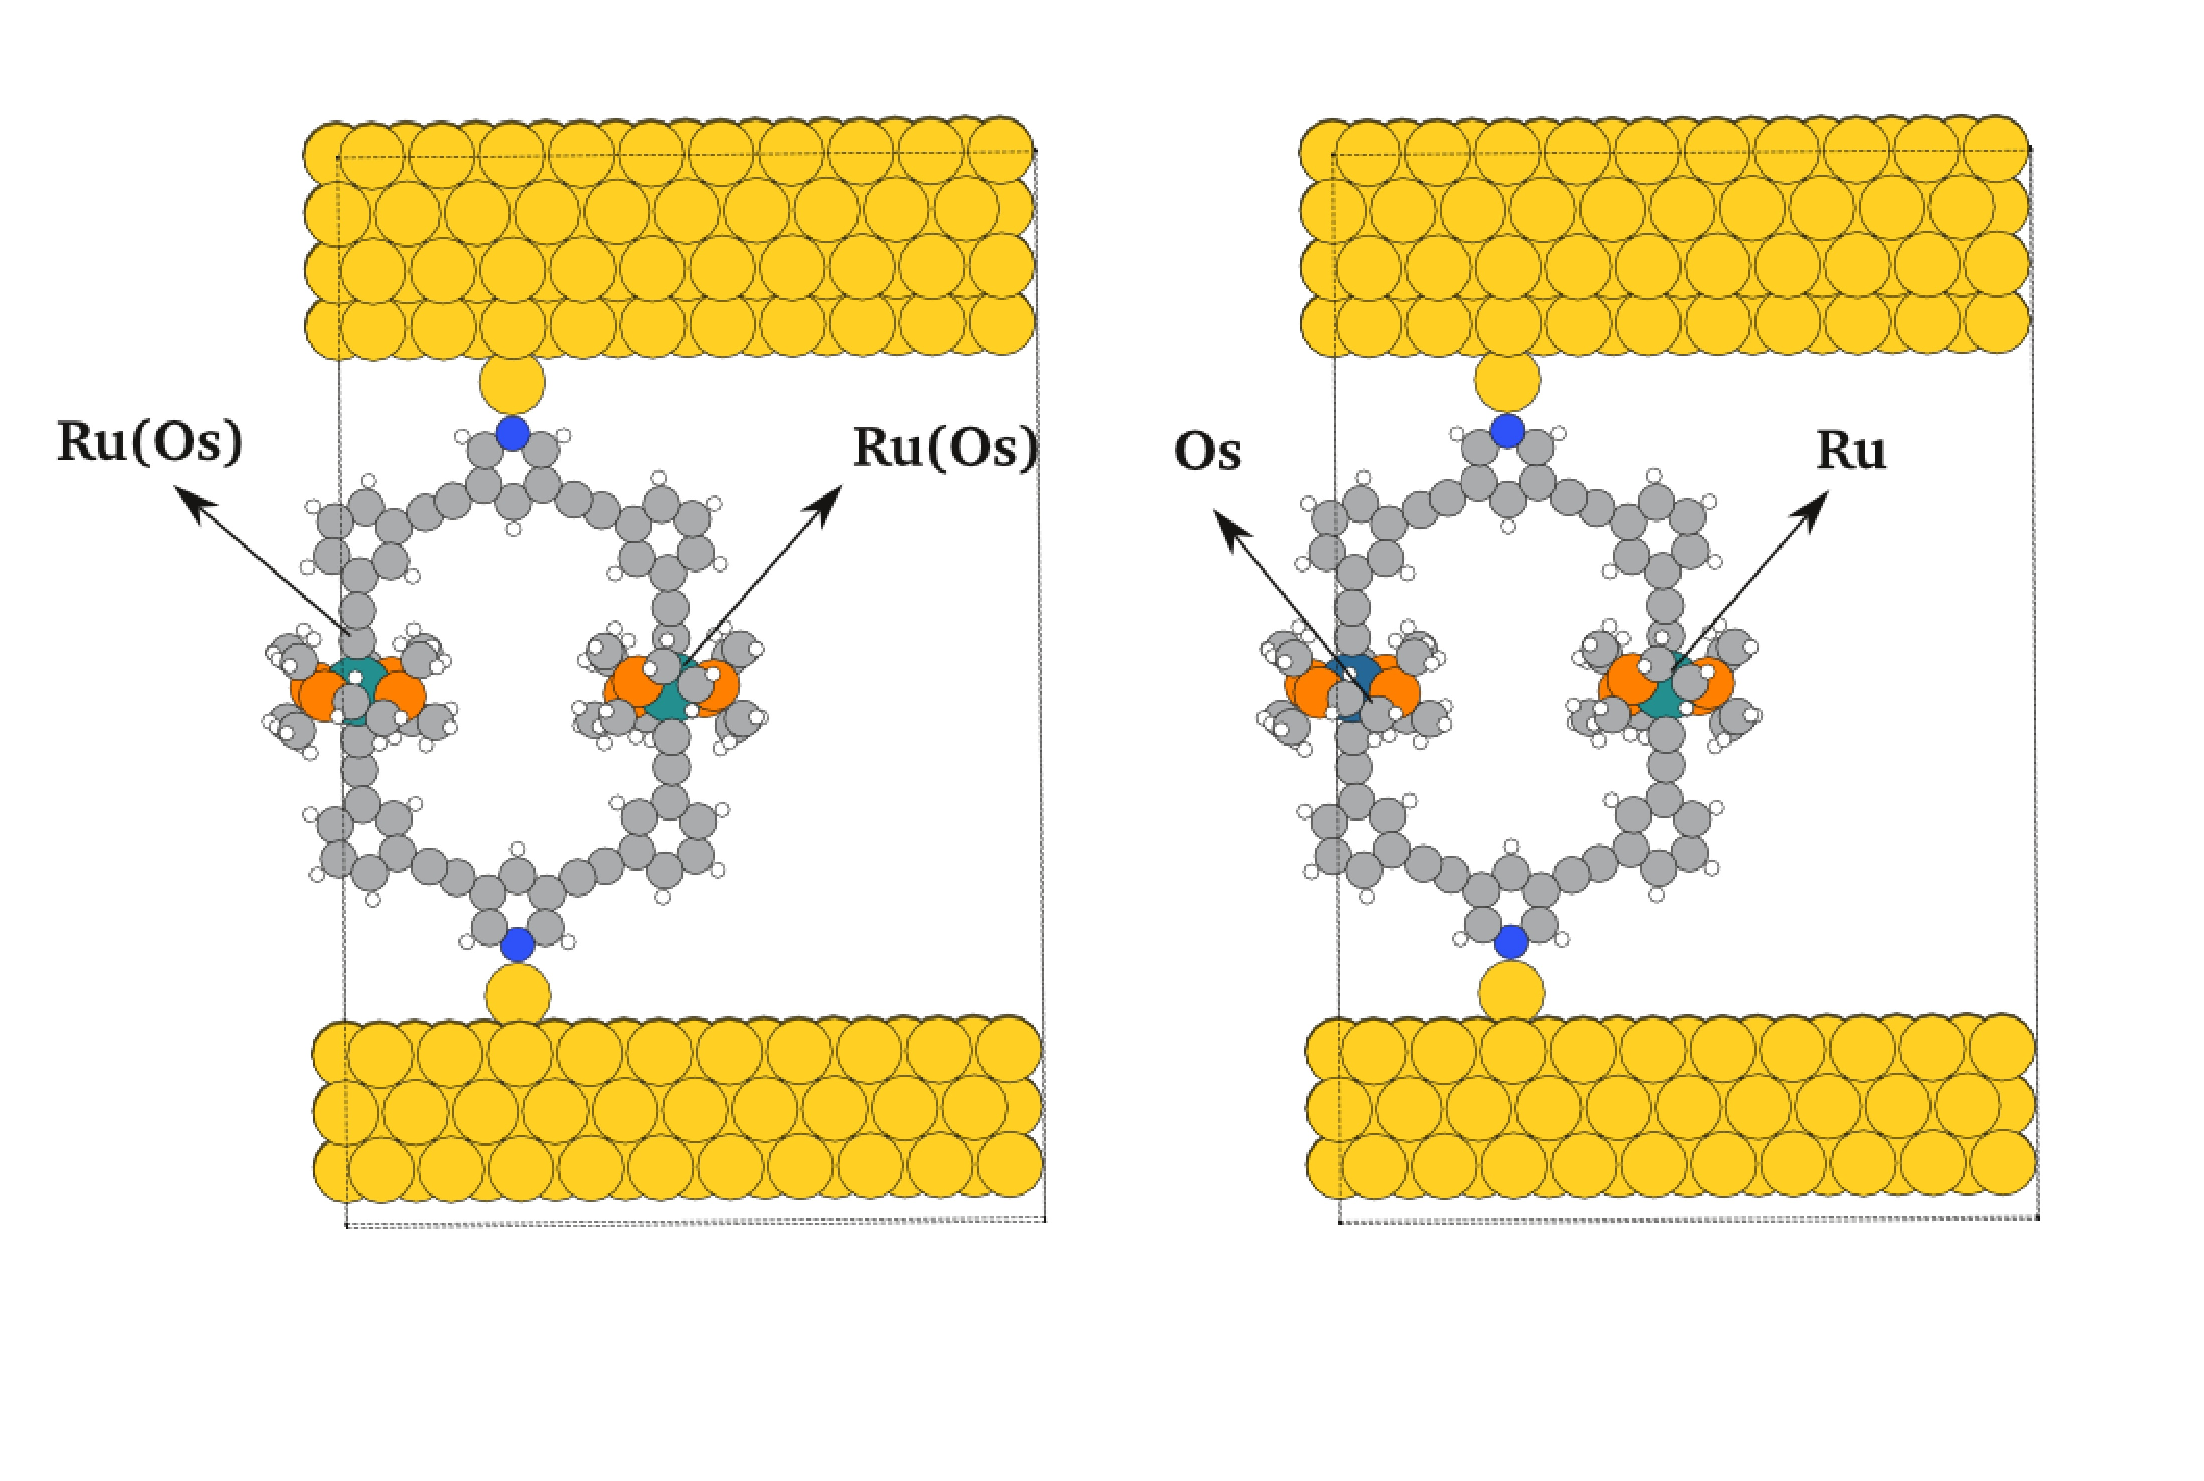
\includegraphics[width=\linewidth,angle=0]{neutral_junction_geo.eps}
\caption{\small Junction structures for the Ru/Ru(Os) molecule.
  \label{Fig.neutral_big_cyclicmol_junctions}} 
\end{center}
\end{figure}
\begin{figure}
\begin{center}
\includegraphics[width=0.8\linewidth,angle=0]{tf_five.png}
\caption{\small Transmission functions for double-branched molecules Ru/Ru (solid red line), Os/Os (solid black line), Ru/Os (green solid line), single branch Ru (dashed red line) and Os (dashed black line) in their neutral states, respectively.
  \label{Fig.big_cyclicmol_tf}} 
\end{center}
\end{figure}
\begin{figure}
\begin{center}
\includegraphics[width=0.8\linewidth,angle=0]{Ru_Ru_neutral_DQI_proof.png}
\caption{\small Transmission functions calculated from NEGF-DFT (red curve) and Larsson's formula (blue and cyan curves) for system Ru/Ru, where the blue curve denotes (HOMO + LUMO)$^2$ and the cyan curve HOMO$^2$ + LUMO$^2$.}
\label{Fig.proof_noDQI}
\end{center}
\end{figure}
In order to clarify whether there are DQI effects in the region of HOMO-LUMO gap, we focus on a simple TB model with a MO basis, where the eigenenergies of the molecular orbitals and their individual coupling values to the electrodes can be obtained by diagonalizing the subspace of the molecule in the we then use Larsson's formula Eq. ~\ref{Larsson's form} ~\cite{lars,lars1,lars2} to calculate the transmission properties $\mathcal{T}(E)$, where only frontier orbitals, namely HOMO and LUMO are included for the proof. 
As one can see from Fig. ~\ref{Fig.proof_noDQI} the contributions from only frontier molecular orbitals HOMO and LUMO can produce the main features (blue curve) from the DFT result (red curve),
From Fig. ~\ref{Fig.proof_noDQI} we see that the contributions from the HOMO and LUMO together, i.e. (HOMO + LUMO)$^2$ (blue curve) are almost identical with the individual contributions (HOMO$^2$ + LUMO$^2$, cyan curve) around E$_F$, which means no DQI between the two MOs is occurring for the system Ru/Ru, and for the other systems Ru/Os, Os/Os, single branch Ru and Os, the conclusion is the same, namely there is no DQI induced minimum in the energy region nearby the Fermi level. The transmission functions from NEGF-DFT for all investigated systems are shown in Fig. ~\ref{Fig.big_cyclicmol_tf}, where
we note that for molecule Ru/Os the peak splitting (green curve) in the occupied region is distinct due to the intrinsic asymmetry by design of the two branches. Up to this point, we would expect that the charging induced upwards energy shift of the HOMO peak will cause conductance fluctuation in Fig ~\ref{Fig.big_cyclicmol_tf}.

We compare the transmission functions for single (red and black dashed lines) and double-branched (red and black solid lines) molecules to illustrate the impact of the number of branches. As we can see the conductance for the Ru (dashed red line) and Ru/Ru (solid red line) molecules are rather similar, and differ only by a factor of about 1.5. While the amount of peaks in the occupied region for the double-branched molecule is higher than the one in the single branch molecule as there are more molecular states coupled to the electrodes for the former. Comparing Os (dashed black line) and Os/Os (solid black line), the conductance for the double-branched molecule is lower by about a factor of 0.6 han for the single molecule. 

The next question is then what is the reason for the absence of DQI in the HOMO-LUMO gap when these molecules share the similar design ideas with the ferrocene molecules we studied before? In order to address this question we move to the AO-FO model we previously used for ferrocene systems ~\cite{Xin2017} and take the single branch Ru molecule as an example due to its representative transmission function, which is very similar to those of the double-branched Ru/Ru, Os/Os and single branch Os molecules. In a first step we include all $p_{\pi}$ AO states of the anchor groups (pyridyl plus the two acetylenic groups) by diagonalizing the subspace of each carbon or nitrogen on these groups and picking the $p_{\pi}$ state.  
For the bridge group two relevant bridge (where we define Ru plus Phosphine ligands and conjugated spacers including acetylenic and benzene groups as the bridge group) FO in the occupied region are considered. Then we diagonalize the two anchor subspaces to get the relevant anchor FO states on both sides. By reducing the number of bridge FO states in the Hamiltonian we finally can minimize the Hamiltonian to the most simple one, which then only contains the three most relevant states, i.e. one FO on each anchor group and one bridge FO, which can be compared with the 3 $\times$ 3 Hamiltonian for the ferrocene systems we discussed before ~\cite{Xin2017}. 
\begin{figure}
\begin{center}
\includegraphics[width=0.6\linewidth,angle=0]{single_Ru_AO_FO_tf.png}
 \caption{\small  Transmission functions for single branch Ru molecule, where red dashed curve is from NEGF-DFT calculation, the three solid lines are obtained from NEGF-TB calculations with eight AO  anchor states ($p_{\pi}$ state of each carbon or nitrogen atom from subdiagonalization) and two bridge states (blue curve), two FOs on each side and two bridge states (green curve), one FO anchor state on each side and one bridge FO (magenta curve).
  \label{Fig.single_Ru_tf_AO_FO}} 
\end{center}
\end{figure}

\subsection{Comparison of a simplified 3 $\times$ 3 Hamiltonian for single branch Ferrocene, Ruthenium molecules} \label{sec:sources}

Based on the scheme we developed in Ref. ~\cite{Xin2017} we use the simplified 3 $\times$ 3 Hamiltonian for a mathematical perspective for explaining the role of the through-space coupling. The systems we investigated here have no DQI feature despite the number of branches even though they are designed similarly to the molecule Fc in ~\cite{Xin2017}, where the most distinct differences here are the molecular length and the type of metal centers. 
In our previous work ~\cite{Xin2017} we found that in order to observe a DQI feature close to E$_{F}$, the through-space coupling value needs to be neither too small nor too big in size so that the DQI feature will not be pushed outside the interesting region as we illustrated in Ref. ~\cite{Xin2017}, where the t$_{D}$ value for DQI occurring near to the position of LUMO peak is -0.023 eV.   
Now we ask for the Ru/Os(PPh$_{2}$)$_{8}$(C$_{2}$H$_{4}$)$_{4}$ bis(pyridylacetylide) molecules: is the length of the molecule causing the through-space coupling between left and right anchors vanish the only reason for the absence of near to the Fermi level? First of all we list the parameters that enter the 3 $\times$ 3 Hamiltonian for the single systems Ru, Os and ferrocene (Fc).
\[
   H_{mol}=
  \left[ {\begin{array}{ccc}
   \varepsilon_{L} & t_{L} & t_{D}\\
   t_{L} & \varepsilon_{B} & t_{R}\\
   t_{D} & t_{R} & \varepsilon_{R}\\
  \end{array} } \right]
\]
\begin {table}
\setlength{\tabcolsep}{1.1em}
\caption {Parameters entering the 3 $\times$ 3 Hamiltonian formed by three FOs ( Fig.~\ref{Fig:3FOs}) for three single branch systems, where all values are given in eV.}\label{tab:couplings}
\begin{center}
    \begin{tabular}{c c c c}
    \hline
    \hline
    %&\multicolumn{1}{ c }{} &\\ 
    
      & Ru & Os & Fc   \\
    \hline
     t$_L$ & -0.026  & -0.023   &  0.27   \\
    \hline
     t$_R$ & 0.019  & 0.019 &  -0.22  \\
    \hline
    t$_D$ & 5.7E-05 & -5.1E-05  & -0.023 \\
    \hline
    $\Delta\varepsilon$ & -1.5 & -1.5  & 0.6 \\
    \hline
    \hline
    \end{tabular}
\end{center}
\end {table}
in Table ~\ref{tab:couplings} we can see the coupling values of t$_{L}$, t$_{R}$ and t$_{D}$ connecting the three FOs (as shown in Fig. ~\ref{Fig:3FOs}) for the three systems Ru, Os and Fc are distinct in the sense that: i) the size of the couplings between anchor and bridge t$_{L/R}$ are one magnitude smaller for Ru and Os than the ones in Fc; ii) the through-spacing coupling t$_{D}$ for the Ru and Os molecules are negligible, iii) the bridge FO we used for the 3 $\times$ 3 Hamiltonian is the highest-lying FO in the occupied region for Ru and Os and it was the the lowest-lying FO in the unoccupied region for Fc, which means
the energy difference between anchor and bridge states $\Delta\varepsilon$ are larger in size and the sign differs compared with the ferrocene molecule. Those differences can be interpreted in the perspective of fragment orbitals in Fig. ~\ref{Fig:3FOs}, where the spatial localization on the anchors in Fig. ~\ref{Fig:3FOs}(a) for the Ru molecule is rather similar to the one in ferrocene molecule (Fig. ~\ref{Fig:3FOs} b)), while t$_{L/R}$, the coupling between anchor where the spatial localization is mainly on pyridyl and the adjacent acetylenic group and bridge FOs where the localization is on the metal center and the neighboring acetylenic spacers are decreased markedly, because in between there is a benzene group separating them as shown in Fig. ~\ref{Fig:3FOs} a). In addition, the increased length also eliminates the direct coupling of the two anchor groups. The bridge state on the Ru molecule is now more delocalized because of the strong conjugation with the adjacent triple bonds, while for Fc the state is more localized on the ferrocene moiety. 
\begin{figure}
    %\captionsetup[subfigure]{labelformat=empty}
    
    \centering
    \subfloat[]{%
     \includegraphics[clip,width=0.8\columnwidth]{singleRu_3FOs.jpeg}%
     }

    \subfloat[]{%
     \includegraphics[clip,width=0.8\columnwidth]{three_FO_orbitals.png}%
     }
    \captionsetup[subfigure]{}
    \caption{\small {Spatial distributions of a)single branch Ru, the anchor FO on each side at 1.3 eV and the bridge FO at -0.2 eV; b) Fc, where the anchor FO on each side at 1.05 eV and the bridge FO at 1.66 eV ~\cite{Xin2017}.}}
     \label{Fig:3FOs}
\end{figure}

Larsson's formula \cite{lars,lars1,lars2} has been used for approximating $\mathcal{T}(E)$ as $\mathcal{T}(E)$ $\sim$ $\Gamma^2 (E)$ for coherent tunneling as we introduced in ~\cite{Xin2017}, where the resulting $\mathcal{T}(E)$ can be normalized ~\cite{lars3} and qualitatively reproduces the curves obtained from NEGF-TB ~\cite{victor}. 
From Larsson's formula,
\begin{equation}
 \Gamma(E) = \sum_{m=1}^{N} \dfrac{\alpha_{m}\cdot\beta_{m}}{E-\varepsilon_{m}} 
 \label{Larsson's form}
\end{equation}
where $\alpha_{m}$, $\beta_{m}$ are the couplings of the molecular state with eigenenergy $\varepsilon_{m}$ to the respective left and right contact states,
a simple mathematical condition can be defined for the energetic positions of DQI induced zeros in $\mathcal{T}(E)$ (when $\mathcal{T}(E)$ $\sim$ $\Gamma^2 (E)$ = 0), i.e. $\Gamma (E)= \gamma_{1}/(E-\varepsilon_{1})+\gamma_{2}/(E-\varepsilon_{2})+\gamma_{3}/(E-\varepsilon_{3})$ also must be zero, where $\gamma_i=\alpha_i \beta_i$ for the three MOs resulting from the simple model. By making use of the specific symmetry properties of the 3 $\times$ 3 Hamiltonian in the model, we can impose $\gamma_1+\gamma_2+\gamma_3$ = 0 and obtain,
\begin{equation}
 E_{0}= \varepsilon_{1} + \frac{1}{1+\frac{\gamma_{3} (\varepsilon_{3}-\varepsilon_{2})} {\gamma_{1} (\varepsilon_{1}-\varepsilon_{2})}}\textperiodcentered{(\varepsilon_{3}-\varepsilon_{1})}
 \label{bigsystems_E0}
\end{equation}
which should be the energy position of the DQI induced minimum $E_{0}$.
Having now established that the parameters t$_{L/R}$, t$_{D}$ and $\Delta \varepsilon$ distinguish the ferrocene molecule Fc with a DQI feature close to the LUMO from the single branch systems Ru and Os, we want to explore the mathematical reasons for the importance of these parameters, where we focus on the comparison of Ru and Fc regarding the three parameters entering the Hamiltonian. 
If we mark the three parameters for ferrocene molecule Fc as F$_{1}$, F$_{2}$, F$_{3}$ and for Ru as R$_{1}$, R$_{2}$, R$_{3}$, there are six combinations for forming a 3 $\times$ 3 Hamiltonian. From these Hamiltonians we calculate the transmission functions for each combination in order to identify the decisive parameter enabling DQI.

Now we approximate the coupling values t$_{L/R}$ with 0.025 eV and 0.25 eV for Ru and Fc, respectively, and plot the transmission functions for the six resulting Hamiltonians based on the different combinations of the three parameters in Fig. ~\ref{tf-six-Hamiltonian}.
\begin{table}
\begin{center}
\setlength{\tabcolsep}{1.1em}
\caption {Three parameters defining the 3 $\times$ 3 Hamiltonian which reproduces the transmission function for the single branch Ru and Fc systems, respectively.}\label{tab:parameters}
    \begin{tabular}{c c c}
    \hline
    \hline
    %&\multicolumn{1}{ c }{} &\\ 
    %\hline
       & Ru & Fc   \\
    \hline
     $\Delta \varepsilon$ (parameter 1) & -1.5 & 0.6 \\
    \hline
     t$_{L/R}$ (parameter 2) & 0.025  & 0.25  \\
    \hline
      t$_{D}$ (parameter 3) &  -5.0E-05  &  -0.023 \\
    \hline
    \end{tabular}
\end{center}
\end {table} 
\begin{figure}
    \begin{center}
    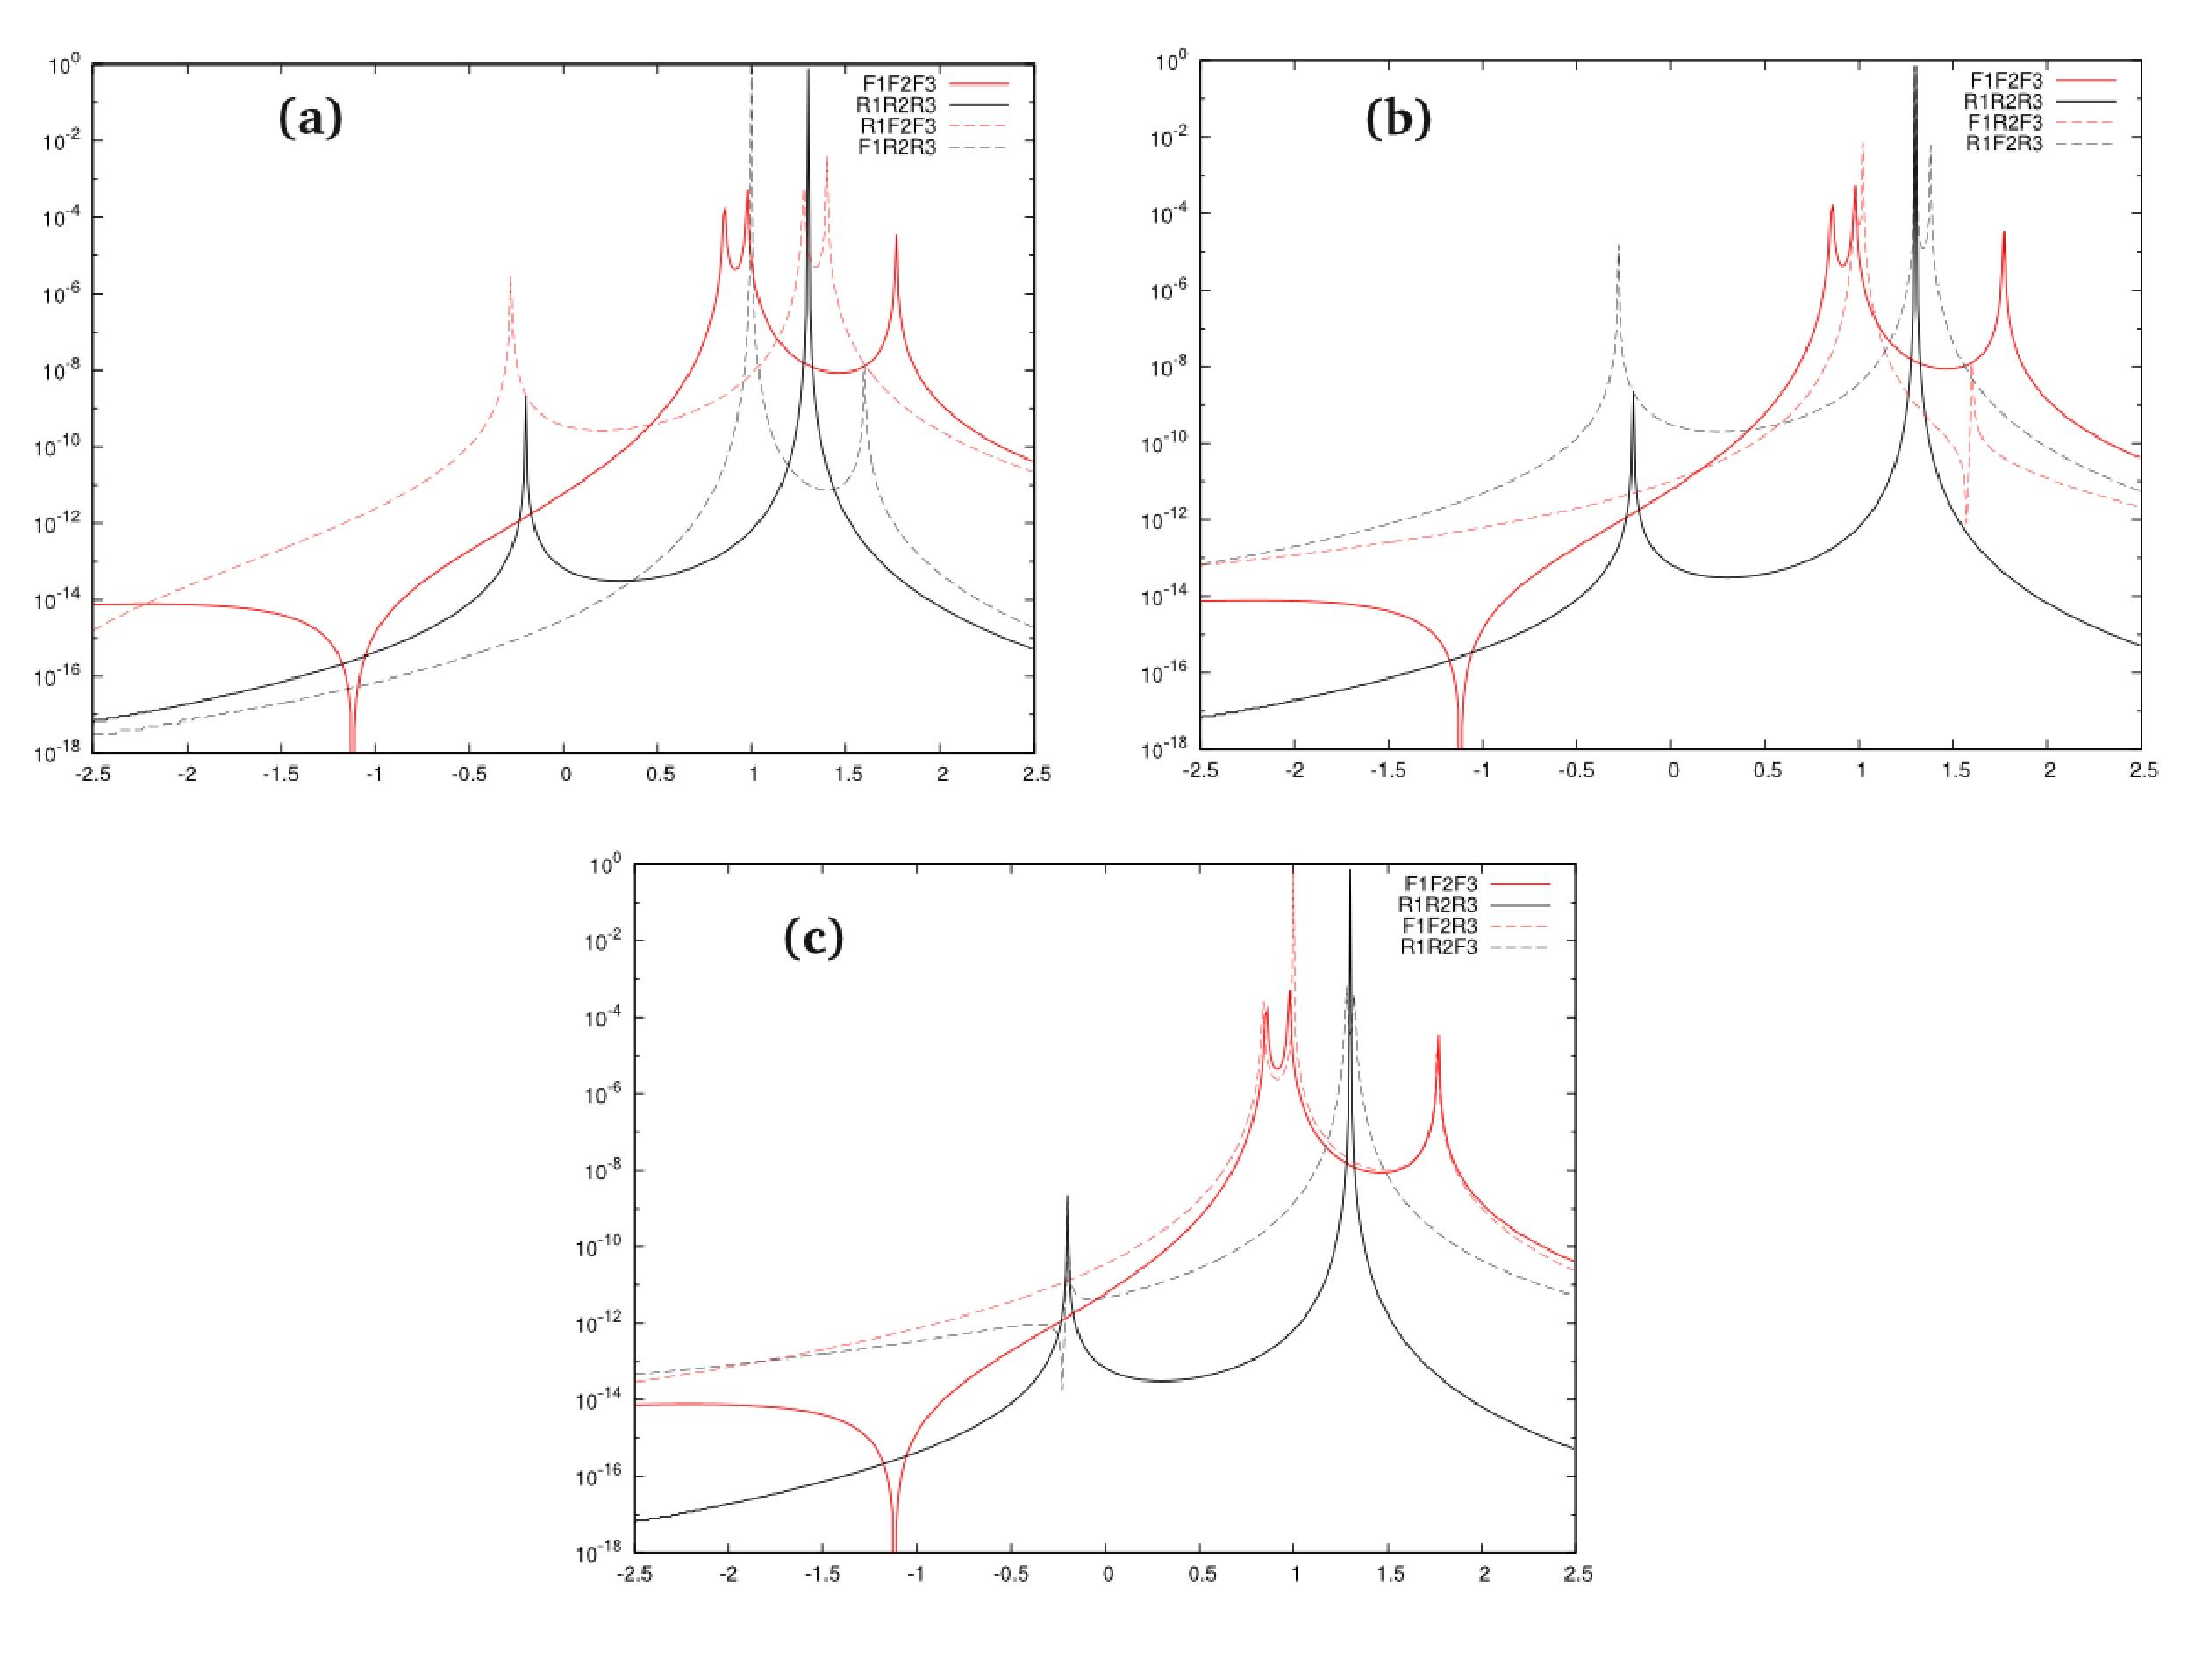
\includegraphics[width=\linewidth,angle=0]{compare_small_H_Ru_Fc-page001.eps}
    \caption{\small Transmission functions of the single branch Ru molecule (black solid line) and the single branch ferrocene molecule (red solid line) a) R$_{1}$F$_{2}$F$_{3}$, meaning replace parameter F$_{1}$ by R$_{1}$ (red dashed line), and F$_{1}$R$_{2}$R$_{3}$ is obtained by replacing R$_{1}$ with F$_{1}$ (black dashed line); b) F$_{1}$R$_{2}$F$_{3}$ (black dashed line) and R$_{1}$F$_{2}$R$_{3}$ (red dashed line); c) F$_{1}$F$_{2}$R$_{3}$ (black dashed line) and R$_{1}$R$_{2}$F$_{3}$ (red dashed line), respectively.}
    \label{tf-six-Hamiltonian}
    \end{center}
\end{figure}
As one can see modifying any one of the three parameters in the Hamiltonian of Fc leads to the disappearance of the DQI feature in the interesting region, which indicates that all three parameters might have a fundamental influence on the DQI absence for Ru in the relevant energy region, meaning that the through-space coupling t$_{D}$ seems to be no longer the only decisive parameter.
We therefore keep two parameters and vary one in a systematic way to see the role each parameter plays.
First of all we keep two parameters t$_{D}$, t$_{L/R}$, and vary $\Delta \varepsilon$, then plot E$_{0}$ versus $\Delta \varepsilon$; secondly we keep $\Delta \varepsilon$ and t$_{D}$, vary t$_{L/R}$ and plot E$_{0}$ from Eq. ~\ref{bigsystems_E0} versus t$_{L/R}$; finally we vary t$_{D}$ while keep the other two parameters constant, and plot E$_{0}$ versus t$_{D}$. The relation between E$_{0}$ and each parameter is illustrated in Fig. ~\ref{E0_ration}. 
\begin{figure}
    \begin{center}
    \includegraphics[width=0.6\linewidth,angle=0]{E0_eps_tL_tD-page001.eps}
    \caption{\small E$_{0}$ versus a) the energy difference $\Delta \varepsilon$ between the anchor and bridge states; b) the coupling value t$_{L/R}$ and c) t$_{D}$ for Ru (black curve) and Fc (red curve), respectively. On each panel, the correct (real) parameter for each system is marked as black dot for Ru and red dot for Fc, i.e. in panel a) black dot ($\Delta \varepsilon$ = -1.5, E$_{0}$ = 12.5) and red dot ($\Delta \varepsilon$ = 0.6, E$_{0}$ = -1.1), in panel b) black dot (t$_{L/R}$ = 0.025, E$_{0}$ = -12.5) and red dot (t$_{L/R}$ = 0.25, E$_{0}$ = -1.1), in panel c) black dot (t$_{D}$ = -0.00005, E$_{0}$ = -12.5) and red dot (t$_{D}$ = -0.023, E$_{0}$ = -1.1) , respectively.}
     \label{E0_ration}
     \end{center}
\end{figure}
From panel (a) we can see that for the Ru system (black curves) where the t$_{D}$ and t$_{L/R}$ values are kept as in table ~\ref{tab:parameters}, E$_{0}$ is always above $\sim$ 12 eV not matter how $\Delta \varepsilon$ varies, i.e. never in the interesting region,
while for the Fc system (red curve) when variable $\Delta \varepsilon$ reaches the real value of Fc, (i.e. 0.6 eV), E$_{0}$ is around -1.1 eV, i.e. close to E$_{F}$ as we also observed in Fig .~\ref{tf-six-Hamiltonian} red solid curve. Besides, for Fc E$_{0}$ covers the range of -3.0 \textemdash {} -1.0 eV along the variable $\Delta \varepsilon$ changes from -2 \textemdash {} 1.5 eV, which means when keeping the t$_{D}$ and t$_{L/R}$ as in the Fc system,  changing $\Delta \varepsilon$ from 0.6 eV to -1.5 eV pushes the DQI minimum away from the Fermi level to $\sim$ -3.0 eV. 
We also plot the relation between E$_{0}$ and t$_{L/R}$ where $\Delta \varepsilon$ and t$_{D}$ are kept as the values in the two respective real systems and show them in Fig.~\ref{E0_ration} b), and find that for system Ru (black curve) E$_{0}$ decreases dramatically when variable t$_{L/R}$ increases, at the real value point -0.00005 eV E$_{0}$ is -12.5 eV, which is out of the interesting region, while for Fc (red curves) we can see the slope of the curve is comparably flat, meaning as long as t$_{L/R}$ is in the range of 0.1 \textemdash {} 0.3 eV, E$_{0}$ is located close to the Fermi level, while when t$_{L/R}$ is smaller than 0.1 eV E$_{0}$ locates above 1.5 eV, which is not within the interesting region anymore.
Finally we plot the relation of t$_{D}$ with E$_{0}$ for the two systems, where we find that for Fc (red curves) the slope of the curve is rather flat compared with the black curve, namely in a rather wide range of variable t$_{D}$ (-0.07 \textemdash {} -0.02 eV), E$_{0}$ is located close to Fermi level, but when t$_{D}$ is above -0.01 eV E$_{0}$ decreases significantly (below -5.0 eV), which means even if one keeps the values of t$_{L/R}$ and $\Delta \varepsilon$ as in the Fc system, as long as t$_{D}$ is above -0.01 eV, where we note that the negative sign is important and refer to our analysis in Ref. ~\cite{Xin2017}, DQI will never within a relevant energy window as is the case for Ru (where t$_{D}$ $\sim$ -0.00005 eV). While in Ru curve (black) when t$_{D}$ reaches -0.023 eV (the real value as in Fc system) E$_{0}$ locates around -0.023 eV which we also found in Fig. ~\ref{tf-six-Hamiltonian} c) black dashed curve, namely it is close to the Fermi level, however, as t$_{D}$ is above -0.001 eV E$_{0}$ decreases
dramatically and always below -5.0 eV which is not in the relevant region anymore, that means in Ru system even the other two parameters $\Delta \varepsilon$ and t$_{L/R}$ are kept as they are, if t$_{D}$ is in the region of -0.01 \textemdash {} -0.001 eV (where the curvature of black curve is rather flat) E$_{0}$ will be close to the Fermi level and we can then observe DQI induced minimum, but when it is above the threshold -0.01 eV, E$_{0}$ is pushed far below the Fermi level. 
 
%\begin{table*}
%\begin{center}
%\setlength{\tabcolsep}{1.1em}
%\caption {Three parameters contained in the small Hamiltonian which produce transmission functions (in Fig. ~\ref{tf-six-Hamiltonian})for single branch $Ru$ and Fc systems, respectively.}\label{tab:parameters}
%    \begin{tabular}{c c c c c c c}
%    \hline
%    \hline
    %&\multicolumn{1}{ c }{} &\\ 
    %\hline
%      & R$_{1}$F$_{2}$F$_{3}$ & F$_{1}$R$_{2}$R$_{3}$& F$_{1}$R$_{2}$F$_{3}$ & R$_{1}$F$_{2}$R$_{3}$ & F$_{1}$F$_{2}$R$_{3}$ & R$_{1}$R$_{2}$F$_{3}$ \\
%    \hline
     
%     t$_D$ & -0.023 & -0.0 & -0.023 & 0.0 & 0.0 & -0.023 \\
%    \hline
%     $E_{0}$ & -2.89 & 1.0E10  & 1.57 & 1.4E12 & 9.2E11 &-0.227\\
%    \hline
%     $\gamma_{3}/\gamma_{1}$ & 20.5  & 0.0034 & -0.0037 & 19.94 &0.21 & 1857.6\\
%    \hline
%     $F_{splitting}$ & -0.08 & -290.0 & -13.26 & -0.05& -4.67 & -0.032\\
%    \hline
%     $F_1$ & -1.57 &  1.6E11  & 0.95 & 8.7E11& 9.9E11 & -0.017 \\
%    \hline
%     $F_2$ & 1.66  & 0.60 & 0.63 & 1.66& 0.927 & 1.52\\ 
%    \hline
%    \hline
%    \end{tabular}
%\end{center}
%\end {table*}
\subsection{Conclusions from the TB analysis}

The summary for this section is that molecules containing metal centers of Ru or Os differ distinctly from the ferrocene molecules we studied before in the relation between molecular structures and the occurrence of DQI effects in electron transmission. 
Strikingly, the most important structural difference of these molecules from the ferrocene molecule Fc is that the length of the molecules we investigate here is larger resulting in the vanishing of through-space coupling, which plays a decisive role. From the plot ~\ref{E0_ration} and the analysis above we conclude that: i) the energy difference between anchor and bridge states $\Delta \varepsilon$ is not a decisive parameter, because as long as we keep the other two parameters (t$_{L/R}$ and t$_{D}$) for Ru we would never observe a DQI minimum in the interesting region (E$_{0}$ is always above 12 eV);
ii) the parameter t$_{L/R}$ is also not a decisive parameter, since E$_{0}$ will be always below -5 eV as long as we keep the other two parameters ($\Delta \varepsilon$ and t$_{D}$) for Ru;
iii) the parameter t$_{D}$ is a decisive parameter, because as long as t$_{D}$ is below the threshold -0.001 eV ($<$ -0.001 eV) for Ru (i.e. keep the other two parameters as in Ru system), one would observe a DQI minimum close to the Fermi level as shown in Fig. ~\ref{E0_ration} c) right panel.


\section{Effect of Charging}\label{Effect of charging}

%The $\Delta$ SCF method allows to define the occupation of particular electronic states of an atom, molecule or solid as a constrain to the self-consistent cycle. 
We used generalized $\Delta$ SCF method for calculating the charging effect in this section, where we put one electron on the chlorine $p$ shell as proposed by Gavnholt \textit{et al}. \cite{deltascf1,deltascf2}. The extra electron is taken from the molecule, in this way the molecule is charged and we keep the neutrality of the entire system.
This approach is based on the generalized $\Delta$ SCF method, and makes use of its flexibility to define the spatial expansion of an orbital forced to contain an electron as an arbitrary linear combination of Bloch states. 

In order to ensure the charge neutrality in the unit cell of the system, which is necessary for a charged junction when applying periodic boundary conditions for electronic-structure calculations, the countercharge to the complex has to be an explicit part of the cell, where we use Cl$^{-}$ as a counterion. 
In our calculations the constrained orbital of chlorine is localized on a single atomic site only, by extracting one electron from the system and inserting it into a predefined orbital in the beginning of every iteration step, the self-consistency cycle progresses as usual, but with the electron density of this particular orbital as a contribution to the external potential. In this way we can fix the electron occupation for the Cl manually. The counterion is added into the junction after the nuclear positions for the neutral complex without Cl is relaxed, then one supplementary electron is constrained to fill the Cl $p$ shell,
which solves the self-interaction problem implicitly and makes this method ideal for charge localization.
Due to its higher electronegativity Cl absorbs an electron from the junction while the overall neutrality of the device region is still maintained as described in detail in Ref. ~\cite{pyridil4}. The junction geometries are shown in Fig. ~\ref{charged-bigmol-junctiond-stru}.

Fig. ~\ref{charged-bigmol-tfs_1}, ~\ref{charged-bigmol-tfs_2} and ~\ref{charged-bigmol-tfs_3} show the transmission functions for each molecule in its neutral and charged states respectively, where we conducted spin-polarized calculations.
The spin-polarization results in two effects in the transmission function: i) MOs move slightly downwards in the energy region, consequently the HOMO is further away from the Fermi level compared with the non-spinpolarized calculations; ii) the splitting of the occupied states nearby the Fermi level becomes more distinct.
The dashed and dot dashed red curves in each panel represent the spin low and high states respectively for the charged system with a distance of 5.2\AA {} between the metal center and Cl atom. As one can see the peak splitting for the two symmetrically built molecules Ru/Ru and Os/Os after charging is distinct as the amount of the charging induced peak shift for the two branches are different, where the branch closer to the chlorine atom have shifted more with respect to the Fermi level, while the MOs on the other branch almost have not been affected by the chlorine charging effect. 
For the asymmetrically built molecule Ru/Os, the peak splitting caused by charging is less distinct, where the peak splitting in the neutral case (black curve) is already rather distinct due to the in-built asymmetry, and charging  does not seem to increase the splitting much further.

The comparison for the three systems under investigation is further analyzed. First of all, for the two identically built systems Ru/Ru and Os/Os the occupied orbital energies HOMO, HOMO-1 and HOMO-2, HOMO-3 are degenerate with energy differences of 0.001 $-$ 0.003 eV, while for Ru/Os the degeneracy is diminished due to the intrinsic asymmetry.  Secondly, for each system in its charged state the energy of the MO on the branch closer to Cl is shifted distinctly compared with the MO on the other branch with spin-polarized results, consequently the asymmetry is introduced, we show the difference for the energies of the MO with respective $d_{xz}$ and $d_{yz}$ symmetries on the branch closer to Cl and on the other branch in Table ~\ref{tab:energydifference}. 
\begin{table*}
\begin{center}
\setlength{\tabcolsep}{1.1em}
\caption {Energy difference (in eV) between branch M$_{1}$ and branch M$_{2}$ in its neutral and corresponding charged states.}\label{tab:energydifference}
    \begin{tabular}{c c c c c c c}
    \hline
    \hline
    &\multicolumn{3}{ c }{d$_{xz}$} &\multicolumn{3}{ c }{d$_{yz}$}\\ 
    \hline
      & Ru/Os & Os/Os & Ru/Ru & Ru/Os & Os/Os & Ru/Ru\\
    \hline
     
     $\Delta \varepsilon_{neutral}$ & 0.120 & 0.001 &  0.002 & 0.090 & 0.001 & 0.003\\
    \hline
     $\Delta \varepsilon_{nospin}$ & 0.017 & 0.015 & 0.012 & 0.022 & 0.026 & 0.027\\
    \hline
     $\Delta \varepsilon_{spin low}$ & 0.121 & 0.064 & 0.098 & 0.096 & 0.094 & 0.090\\
    \hline
     $\Delta \varepsilon_{spin high}$ & 0.184 & 0.159 & 0.157 & 0.123 & 0.131 & 0.115\\
    \hline

%    \hline
    \end{tabular}
\end{center}
\end{table*} 
Thirdly, in the non-spinpolarized calculations the peaks for all systems are shifted upwards compared with the corresponding neutral case, while in the spin-polarized results the HOMO-2, HOMO-3 peaks of Os/Os (Cl) are shifted downwards and for Ru/Os (Cl) in spin-low case the four peaks are shifted slightly downwards. One more notable thing is that in the asymmetrically built system Ru/Os, the amount of the shift induced by charging is smaller than the other two systems as we mentioned above, we can clearly see the distance of the peaks in black curve and red dot-dashed curve in Fig. ~\ref{charged-bigmol-tfs_1} is smaller than the peak distance in Fig. ~\ref{charged-bigmol-tfs_2} and Fig. ~\ref{charged-bigmol-tfs_2}.
\begin{figure*}
 \begin{center}
    \includegraphics[width=1.\linewidth,angle=0]{LFT.jpg}
    \caption{\small Electron occupation in the Ru $d$ orbitals.}
\label{LFT}
\end{center}
\end{figure*}
The metal centers in the investigated systems are stabilized by four donor ligands as shown in Fig. ~\ref{Fig.chemicalstru}, which suggests a tetragonal ligand field where the orbitals splittings with different energetic ordering $d_{x^2-y^2}$ and $d_{xz}$, $d_{yz}$ are found by DFT calculations \cite{J.Bendix 2005}.
According to Ligand field theory ~\cite{LFT}, for an octahedral field with Jahn Teller distortion, e$_{g}$ orbitals $d_{x^2-y^2}$ and $d_{z^2}$ are in higher energy levels, the three $d$ orbitals $d_{xz}$, $d_{yz}$ and $d_{xy}$ are in lower energy levels. We find that the peaks in the occupied region close to the Fermi level are contributed mostly from the two $d$ orbitals with $d_{xz}$, $d_{yz}$ symmetries, while the $d_{xy}$ lies far lower to the Fermi level, we conclude that for Ru/Ru and Os/Os compounds the fast channel (coherent tunneling) is attributed to the delocalized HOMO state $d_{yz}$ and for Ru/Os it is attributed to $d_{xz}$, which is also found in the work ~\cite{Georg 2016}. 
For the systems investigated here one can see from the eigenstates for the $d$-orbitals $d_{xz}$ and $d_{yz}$, they are fully occupied for all systems when in its neutral state while for charged states one electron is supposed to be taken to Cl $p$ orbital so the Ru (\rom{2}) with six $d$- electrons is now Ru (\rom{3}) with five $d$- electrons and the electron occupation according to Ligand field theory is shown in Fig. ~\ref{LFT}, meaning after charging one of the $d_{xz}$ and $d_{yz}$ is singly occupied which complies with Hund's rule. The single occupation leads to a spin-polarization of the Kohn-Sham orbitals thus the energetic ordering for the relevant MOs changes. 
As we can see from Fig. ~\ref{charged-bigmol-tfs_2} and ~\ref{charged-bigmol-tfs_3} the evolution from neutral states to the charged states, the HOMO-1 and HOMO-2 change the energetic ordering sequence for Ru/Ru and Os/Os due to the degeneracy in the their neutral states.  While that is not the case for Ru/Os, i.e. for Ru/Os the energetic ordering of HOMO, ... HOMO-3 remains the same as the corresponding neutral case after charging (as shown in Fig. ~\ref{charged-bigmol-tfs_1}).
\begin{figure}[h]
    \begin{center}
    \includegraphics[width=\linewidth,angle=0]{charged_junction_stru.jpg}
    \caption{\small Junction geometries for two neighboring cells in the periodic setup for the scattering region of double branched Ru/Os (Cl) in a distance of 5.2 \AA{}.}
    \label{charged-bigmol-junctiond-stru}
    \end{center}
\end{figure}
%\begin{figure}[h]
% \begin{center}
 %   \includegraphics[width=0.6\linewidth,angle=0]{double_branched_HOMOs_neutral_charged.eps}
 %   \caption{\small Spatial distributions of the four MOs directly below E$_F$ (HOMO,...,HOMO-3) for the big cyclic molecule Ru/Ru in its a) neutral state; b) chlorine charged state.}
%    \label{Fig:HOMOs}
 %   \end{center}
%\end{figure}
\begin{figure*}
    \begin{center}
    \includegraphics[width=\linewidth,angle=0]{Ru_Os_spin_effect-page001.eps}
    \caption{\small Four relevant occupied orbitals and transmission functions for Ru/Os(Cl) with spin and without spin-polarization in a distance of 5.2 \AA {}, respectively. Where the black and red solid curves are the respective neutral and charged states, while the dashed and dot dashed curves in each panel mean spin low state and spin high state, respectively.}
    \label{charged-bigmol-tfs_1}
    \end{center}
\end{figure*}
\begin{figure*}
    \begin{center}
    \includegraphics[width=\linewidth,angle=0]{Os_Os_spin_effect-page001.eps}
    \caption{\small Four relevant occupied orbitals and transmission functions for Os/Os(Cl) with spin and without spin-polarization in a distance of 5.2 \AA {}, respectively. Where the black and red solid curves are the respective neutral and charged states, while the dashed and dot dashed curves in each panel mean spin low state and spin high state, respectively. }
    \label{charged-bigmol-tfs_2}
    \end{center}
\end{figure*}
\begin{figure*}
    \begin{center}
    \includegraphics[width=\linewidth,angle=0]{Ru_Ru_spin_effect-page001.eps}
    \caption{\small Four relevant occupied orbitals and transmission functions for Ru/Ru(Cl) with spin and without spin-polarization in a distance of 5.2 \AA {}, respectively. Where the black and red solid curves are the respective neutral and charged states, while the dashed and dot dashed curves in each panel mean spin low state and spin high state, respectively. }
    \label{charged-bigmol-tfs_3}
    \end{center}
\end{figure*}

We list the conductance of the neutral and charged states for each system, as well as the partial charge on molecules where we intend to see the asymmetry induced by charging. As we can see from table ~\ref{tab:charge and G} the asymmetry induced by Cl charging effect is quite distinct compared with the corresponding neutral molecules, while the conductance of the charged systems changes only slightly since the energy shifts of the peaks in the occupied region are small and the conductance is dominated by those peaks in the occupied region. We plot the spatial localization for the orbitals in the occupied region of both neutral and charged systems.
As one can see from Fig. ~\ref{charged-bigmol-tfs_1}, ~\ref{charged-bigmol-tfs_2} and ~\ref{charged-bigmol-tfs_3} the d$_{xz}$ and d$_{yz}$ orbitals of the metal hybridize with the organic ligands resulting in the delocalization, which contributed to the conductance. 
\begin {table}[h]
\setlength{\tabcolsep}{0.5em}
\caption {Partial charges in units of fractions of 1 e as obtained from a Bader analysis ~\cite{bader} for the neutral and charged molecules, where M$_{1}$ and M$_{2}$ denote the branch containing the metal center closer to and further away from the chloride ion, respectively. The conductance G for all molecules as defined by $\mathcal{T}(E_{F})$ is given in units of G$_{0}$.} \label{tab:charge and G}
\begin{center}
    \begin{tabular}{c c c c}
    \hline
    \hline
     & M$_{1}$ & M$_{2}$ & G \\ \hline
    \hline
    Ru/Os (neutral)  & 0.0345 & 0.0378 & 4.57\texttimes 10$^{-9}$ \\
    \hline
    Ru/Os (d$_{Cl-M}$=5.2\AA)  & -0.710 & -0.173  & 3.41\texttimes 10$^{-9}$ \\
    \hline
    \hline
    Os/Os (neutral)  & 0.036 & 0.036 & 4.61\texttimes 10$^{-9}$ \\
    \hline
    Os/Os (d$_{Cl-M}$=5.2\AA) & -0.230 & -0.653  & 1.84 \texttimes 10$^{-8}$ \\
    \hline
    \hline
    Ru/Ru (neutral)  & 0.038 & 0.037 & 2.41\texttimes 10$^{-9}$ \\
    \hline
    Ru/Ru (d$_{Cl-M}$=5.2\AA)  & -0.662 & -0.208 & 2.21 \texttimes 10$^{-8}$ \\
    \hline
    \hline
    \end{tabular}
\end{center}
\end{table}
%
\section{Summary}\label{sec:summary}

In this study we investigated the potential use of branched molecules containing different metal centers in two branches as molecular transistors where the switching would be achieved by a redox process allowing to alternate between an ON and an OFF state. We did not find a DQI effect in electron transmission for these branched molecules, neither in their neutral nor in their charged states. By comparing our results with a previously studied ferrocene compound, we found that due to the increased molecular length, the decisive parameter over-space coupling t$_{D}$ incapacitates the DQI induced minimum appear in the relevant energy region.

The charging effect on these cyclic molecules is not pronounced regarding the conductance change since from the transmission curves (Fig. ~\ref{charged-bigmol-tfs_1}, ~\ref{charged-bigmol-tfs_2} and ~\ref{charged-bigmol-tfs_3}) the upward shift in energy induced by charging is small. The splitting peaks in the solid and dashed red curves in Fig.~\ref{charged-bigmol-tfs_2} and ~\ref{charged-bigmol-tfs_3} indicate the charging effect on one branch (closer to Cl) is more significant than the other. Charging induced asymmetry for these cyclic molecules is rather distinct (see table ~\ref{tab:charge and G}), especially for the asymmetrically built molecule Ru/Os(Cl).


\newpage
\bibliographystyle{apsrev}
\bibliographystyle{apsrev}

\begin{thebibliography}{}

\bibitem{ratner} M. Ratner, \textit{Nature Nanotech.} \textbf{8}, 378 (2013).
\bibitem{loertscher} E. L\"{o}rtscher, \textit{Nature Nanotech.} \textbf{8}, 381 (2013).
\bibitem{Thygesen 2005}K.S. Thygesen and K.W. Jacobsen, \textit{Chem. Phys.} \textbf{319}, 111 (2005).
\bibitem{C. Joachim 1995}C. Joachim, J.K. Gimzewski, R.R. Schlittler and C. Chavy, \textit{Phys. Rev. Lett.} \textbf{74}, 2102 (1995).
\bibitem{M. A. Reed 1997}M.A. Reed, C. Zhou, C.J. Muller, T.P. Burgin and J.M. Tour,
\textit{Science} \textbf{278}, 252 (1997).
\bibitem{J. Reichert 2002}J. Reichert, R. Ochs, D. Beckman, H.B. Weber, M. Mayor and
H.v. L\"{o}hneysen, \textit{Phys. Rev. Lett.} \textbf{88}, 176804 (2002).
\bibitem{R. H. M. Smit 2002}R.H.M. Smit, Y. Noat, C. Untiedt, N.D. Lang, M.C. van Hemert,
and J.M. van Ruitenbeek, \textit{Nature (London)} \textbf{419}, 906 (2002).
\bibitem{mayor}M. Mayor, H. B. Weber, J. Reichert, M. Elbing, C. von H\"{a}nisch, D. Beckmann and M. Fischer, \textit{Angew. Chem. Int. Ed.} \textbf{42}, 5834 (2003).
\bibitem{lambert1}C. J. Lambert, \textit{Chem. Soc. Rev.} \textbf{44}, 875 (2015).

\bibitem{graphical1}R. Stadler, S. Ami, M. Forshaw and C. Joachim, \textit{Nanotechno.} \textbf{15}, S115 (2004).

\bibitem{memory}R. Stadler, M. Forshaw and C. Joachim, \textit{Nanotechnology} \textbf{14}, 138 (2003).
\bibitem{fano}R. Stadler and T. Markussen, \textit{J. Chem. Phys.} \textbf{135}, 154109 (2011).
\bibitem{lambert2}C. M. Finch, V. M. Garcia-Suarez and C. J. Lambert, \textit{Phys. Rev. B} \textbf{79}, 033405 (2009).
\bibitem{molen}C. M. Guedon, H. Valkenier, T. Markussen, K. S. Thygesen, J. C. Hummelen and S. J. van der Molen, \textit{Nat. Nanotechnol.} \textbf{7}, 305 (2012).
\bibitem{tim}M. S. Inkpen, T. Albrecht and N. J. Long, \textit{Organometallics} \textbf{32}, 6053 (2013).
\bibitem{hopping}G. Kastlunger and R. Stadler, \textit{Phys. Rev. B} \textbf{91}, 125410 (2015).
\bibitem{Georg 2015}G. Kastlunger and R. Stadler, \textit{Phys. Rev. B} \textbf{91}, 125410 (2015).
\bibitem{Schwarz 2015}F. Schwarz, G.Kastlunger, F. Lissel, H. Riel, K. Venkatesan, H. Berke, R. Stadler and E. L\"{o}rtscher, \textit{Nat Nanotechnol}, \textbf{11}, 170–176 (2016).
\bibitem{Xin2017}X. Zhao,G. Kastlunger, and R. Stadler, \textit{Phys. Rev. B} \textbf{96}, 085421 (2017).
\bibitem{M.Brandbyge 2002}M. Brandbyge, J.-L. Mozos, J. Taylor, K. Stokbro, \textit{Phys. Rev. B}, \textbf{65}, 165401 (2002).
\bibitem{Y.Xue 2002}Y. Xue, S. Datta, M. A. Ratner, \textit{Chem. Phys.}, \textbf{281}, 151 (2002).
\bibitem{A.R.Rocha 2005}A.R. Rocha, V M. Garcia-Suarez, S.W. Bailey, C.J. Lambert, J. Ferrer, S. Sanvito, \textit{Nat. Mater.}, \textbf{4}, 335 (2005).
\bibitem{kristian}K. S. Thygesen and K. W. Jacobsen, \textit{Chem. Phys.}, \textbf{319}, 111 (2005).
\bibitem{pbe}J. P. Perdew, K. Burke and M. Ernzerhof, \textit{Phys. Rev. Lett.} \textbf{77}, 3865 (1996).
\bibitem{lcao}A.H. Larsen, M. Vanin, J.J. Mortensen, K.S. Thygesen and K.W. Jacobsen, \textit{Phys. Rev. B}, \textbf{80}, 195112 (2009).
\bibitem{pyridil1}R. Stadler, K. S. Thygesen and K. W. Jacobsen, \textit{Phys. Rev. B} \textbf{72}, 241401(R) (2005).
\bibitem{pyridil3}R. Stadler, \textit{Phys. Rev. B} \textbf{80}, 125401 (2009).
\bibitem{victor}X. Zhao, V. Geskin and R. Stadler, \textit{J. Chem. Phys.} \textbf{146}, 092308 (2017).
\bibitem{lars}S. Larsson, \textit{J. Am. Chem. Soc.} \textbf{103}, 4034 (1981).
\bibitem{lars1}M. A. Ratner, \textit{J. Phys. Chem.} \textbf{94}, 4877 (1990).
\bibitem{lars2}G. Kastlunger and R. Stadler, \textit{Phys. Rev. B} \textbf{89}, 115412 (2014).
\bibitem{lars3}P. Sautet and M.-L. Bocquet, \textit{Phys. Rev. B} \textbf{53}, 4910 (1996).
\bibitem{J.Bendix 2005}J. Bendix, T. Birk, T. Weyhermuller, \textit{Dalton Trans.}, 2737 (2005).
\bibitem{LFT}C. E. Sch\"{a}ffer, C. Anthon and J. Bendix. \textit{Coordination Chemistry Reviews, Theory and Computing in Contemporary Coordination Chemistry} \textbf{253}, 575 (2009).

\bibitem{Georg 2016}F. Schwarz, G. Kastlunger, F. Lissel, C. Egler-Lucas, S.N. Semenov, K. Venkatesan, H. Berke, R. Stadler and E. L\"{o}rtscher, \textit{Nat. Nanotech.} \textbf{11},170 (2016).

\bibitem{pyridil4}G. Kastlunger and R. Stadler, \textit{Phys. Rev. B}, \textbf{88}, 035418 (2013).
\bibitem{deltascf1}J. Gavnholt, T. Olsen, M. Engelund and J. Schi\o{}tz, \textit{Phys. Rev. B}, \textbf{78}, 075441 (2008).
\bibitem{deltascf2}T. Olsen, J. Gavnholt and J. Schi\o{}tz, \textit{Phys. Rev. B}, \textbf{79}, 035403 (2009).
\bibitem{bader}W. Tang, E. Sanville and G. Henkelman, \textit{J. Phys. Condens. Matter} \textbf{21}, 084204 (2009).
 
\end{thebibliography}


\end{document}

